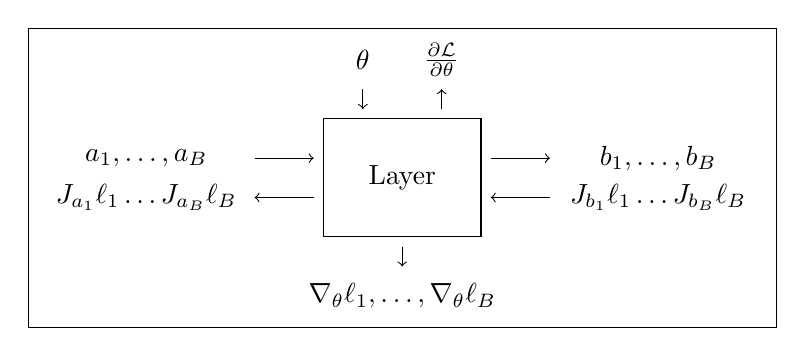
\begin{tikzpicture}


\draw  (-4.75,1.9) rectangle (4.75,-1.9);
\draw  (-1,0.75) rectangle (1,-0.75);
\node (v5) at (1,0.25) {};
\node (v6) at (2,0.25) {};
\node (v9) at (1,-0.25) {};
\node (v10) at (2,-0.25) {};
\node (v11) at (-1,-0.25) {};
\node (v12) at (-2,-0.25) {};
\node (v13) at (-2,0.25) {};
\node (v14) at (-1,0.25) {};
\node (v2) at (-0.5,0.75) {};
\node (v1) at (-0.5,1.25) {};
\node (v4) at (0.5,1.25) {};
\node (v3) at (0.5,0.75) {};
\node (v7) at (0,-0.75) {};
\node (v8) at (0,-1.25) {};
\draw[->] (v1) edge (v2);
\draw[->]  (v3) edge (v4);
\draw[->]  (v5) edge (v6);
\draw[->]  (v7) edge (v8);
\draw[<-]  (v9) edge (v10);
\draw[->]  (v11) edge (v12);
\draw[->]  (v13) edge (v14);
\node at (0,0) {Layer};
\node at (-0.5,1.5) {$\theta$};
\node at (0.5,1.5) {$\frac{\partial \mathcal{L}}{\partial \theta}$};
\node at (3.25,0.25) {$b_1, \ldots, b_B$};
\node at (3.25,-0.25) {$J_{b_1} \ell_1 \ldots J_{b_B} \ell_B$};
\node at (-3.25,0.25) {$a_1, \ldots, a_B$};
\node at (-3.25,-0.25) {$J_{a_1} \ell_1 \ldots J_{a_B} \ell_B$};
\node at (0,-1.5) {$\nabla_\theta \ell_1, \ldots, \nabla_\theta \ell_B$};
\end{tikzpicture}